\documentclass{beamer} 
%\documentclass[handout]{beamer} 

% Michael Maier, 2016.
% CC-0

\usepackage[utf8]{inputenc}
\usepackage[ngerman]{babel}

\title{Routing für Menschen mit Behinderung mit OpenStreetMap - wheelroute.at}
\author{Michael Maier \textless Michael.Maier@student.tugraz.at\textgreater} 
\date{30. November 2016} 

\usetheme{Antibes}

\newcommand{\boldm}[1] {\mathversion{bold}#1\mathversion{normal}}

\hypersetup{colorlinks=true,urlcolor=blue,linkcolor=white}

%\usebackgroundtemplatei{
%
\includegraphics[width=\paperwidth,
%height=0.8\paperheight]{mag_map.png}
%}

\begin{document}

%\maketitle

\begin{frame} 


\begin{figure}
  \centering
  
\includegraphics[width=.4\textwidth]{mag_map.png}
\end{figure}

\begin{center}
\Huge{Routing für Menschen mit Behinderung\\}
\end{center}

\begin{center}
\Large{\emph{mit OpenStreetMap}}
\end{center}

\end{frame}


\section{Einleitung}

\begin{frame}{Vorstellung}

  \begin{itemize}
    \item Michael Maier \textless \href{mailto:Michael.Maier@student.tugraz.at}{Michael.Maier@student.tugraz.at}\textgreater
    \item Student an der TU Graz (Telematik)
\vspace{0.3cm}
    \item OpenStreetMap als Hobby seit 2010
    \item Leite den Grazer OSM-Stammtisch seit Mai 2011
\vspace{0.3cm}
    \item Freiberuflich OSM-Aufträge und Consulting
  \end{itemize}
\end{frame}

\begin{frame}{OpenStreetMap}


  \begin{itemize}
        \item OpenStreetMap (OSM) ist eine freie Weltkarte nach dem Wiki-Prinzip "`Wikipedia der Karten"'
          \pause
            \item Entsteht aus der Arbeit von \textgreater 3\,M Hobbykartografen "`\emph{Mapper}"'
          \end{itemize}

           \begin{center}
              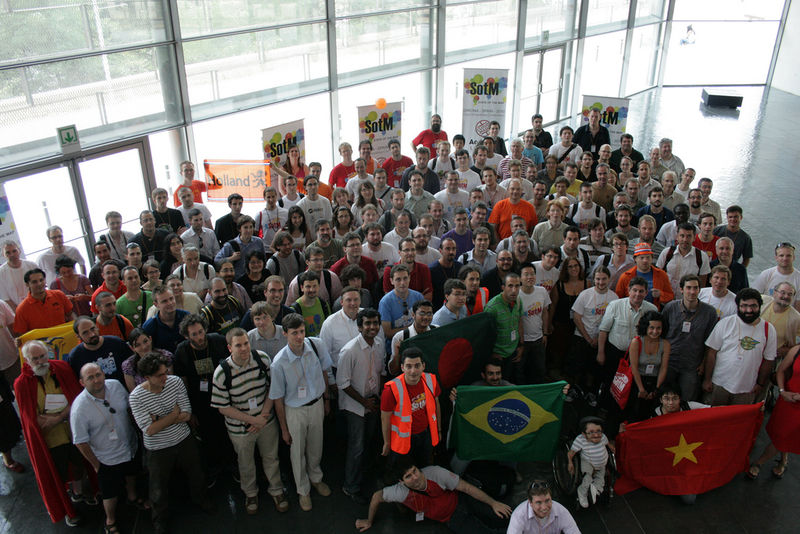
\includegraphics[width=4.5cm]{sotm.jpg}
               \end{center}

             \pause
  Wheelmap.org baut auf OSM auf!

\end{frame}

\section{Projekt wheelroute.at}

\begin{frame}{Ziel des Projektes}

    \begin{itemize}
       \item Barrierefreiheit im Innenstadtbereich überprüfen

         \pause

      \vspace{1cm}

      \item Rückmeldung an die Stadt Graz, wo Prioritäten für Verbesserungen liegen
    \end{itemize}


\end{frame}

\begin{frame}{Zielgebiet}

  \begin{columns}[c]
    \begin{column}[T]{.6\textwidth}
      \begin{center}
      \vspace{-1cm}
      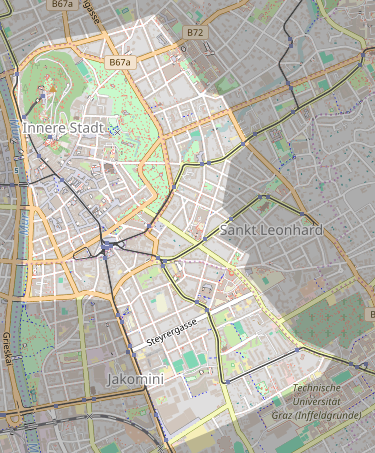
\includegraphics[width=6cm]{gebiet.png}
      \end{center}
    \end{column}
    \begin{column}[T]{.4\textwidth}
      \begin{itemize}
            \item 3,2 km$^2$
            \item Innere Stadt bis Karl-Franzens-Uni
    \item       Karl-Franzens-Uni bis TU (Inffeld)
  \item       Jakominiplatz bis Messe
    \vspace{1cm}
  \item       Nach demselben Schema wurde vor 3~Jahren die Stadt Gleisdorf erfasst.
    \end{itemize}

    \end{column}
  \end{columns}

\end{frame}

\begin{frame}{Was wurde erfasst?}

    \begin{itemize}
      \item Bordsteinkanten-Höhen
      \item Steigungen, Querneigungen
      \item Breiten
      \item Oberfläche
      \item Fußgängerampeln und taktile Bodenmarkierungen
    \end{itemize}


\end{frame}

\begin{frame}{Wie wurde erfasst?}
    \begin{itemize}
      \item Rollmaß für Breiten und Kantenhöhen
      \item Digitale Wasserwaage für Steigungen und Querneigungen
      \item Papier \& Bleistift
      \item Fotos bei kritischen Stellen
    \end{itemize}

\end{frame}

\begin{frame}{Wer hat erfasst?}

  Dank für Mithilfe gilt:
  \begin{itemize}
        \item Christian Pani (Hand-Rolli)
        \item Hanna Hoefer (Hand-Rolli)
        \item Christian Grübl (E-Rolli)
  \end{itemize}
            \vspace{1cm}

  \pause
  Der Großteil durch mich selbst zu Fuß/Fahrrad.

\end{frame}



\section{Ergebnisse}

\subsection{Routing}

\begin{frame}{}

  \begin{columns}[c]
    \begin{column}[T]{.6\textwidth}
      \begin{center}
      \vspace{-1cm}
      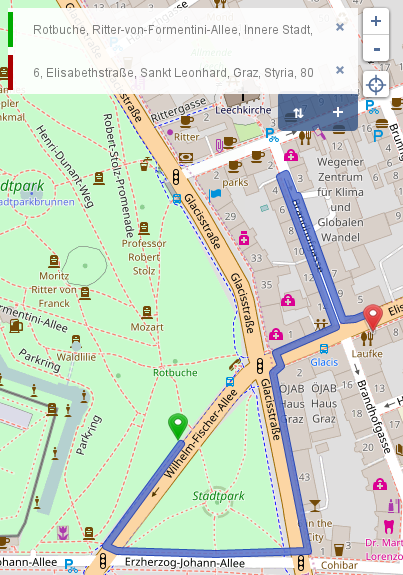
\includegraphics[width=5.5cm]{routing1_normal.png}
      \end{center}
    \end{column}
    \begin{column}[T]{.4\textwidth}
      www.wheelroute.at
      \begin{itemize}
      \vspace{1cm}
        \item Routingservice im Beta-Stadium (\href{http://mm.linuxtage.at/osm/routing/wheelchair-normal/?z=17\&center=47.072643\%2C15.452845\&loc=47.073045\%2C15.446059\&loc=47.073841\%2C15.448145\&hl=en\&ly=\&alt=\&df=\&srv=}{Link})
              \pause
      \vspace{1cm}
            \item 3 Profile:
              \begin{itemize}
                \item Hand-Rolli
                \item E-Rolli
                \item Sportliche Fahrer
          \end{itemize}
        \end{itemize}

    \end{column}
  \end{columns}

\end{frame}

\subsection{Hinderniss-Karte}

\begin{frame}{}

  \begin{columns}[c]

    \begin{column}[T]{.6\textwidth}
      \begin{center}
      \vspace{-0.3cm}
      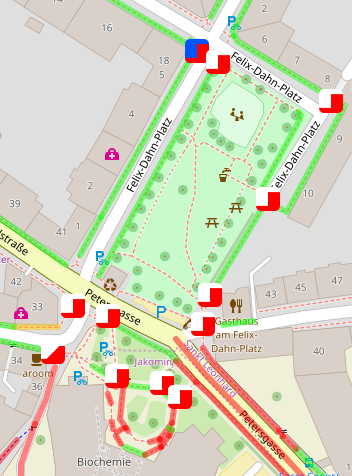
\includegraphics[width=5.5cm]{hindernisse.png}
      \end{center}

    \end{column}
    \begin{column}[T]{.4\textwidth}

      \begin{itemize}
      \vspace{1cm}
          \item Farbdarstellung mit klickbaren Elementen (\href{http://species.github.io/wheelchair-obstacles/normal.html\#18/47.06588/15.45369}{Link})

      \vspace{1cm}

            \item 4 Verschiedene Karten:

              \begin{itemize}
                \item Hand-Rolli
                \item E-Rolli
                \item Sportliche Fahrer
                \item Kaputte Ampeln
              \end{itemize}
        \end{itemize}

    \end{column}
  \end{columns}

\end{frame}

\begin{frame}{Fotos}

  \begin{columns}[c]
    \begin{column}[T]{.6\textwidth}

      \begin{center}
      \vspace{-1cm}
      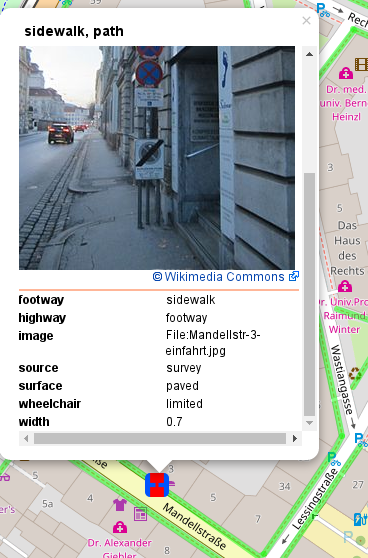
\includegraphics[width=5.5cm]{Fotos-screenie.png}
      \end{center}

    \end{column}
    \begin{column}[T]{.4\textwidth}

      \begin{itemize}
        \vspace{1cm}
        \item Blaue Icons haben ein Foto.
        \vspace{1cm}
        \item Fotos wurden auf Wikimedia Commons gestellt.
        \end{itemize}

    \end{column}
  \end{columns}

\end{frame}

\begin{frame}{Statistik}

  Was haben wir gefunden?

      \begin{itemize}
        \item 65 (teilweise) defekte Ampeln
        \item 137 nicht abgesenkte Gehsteigkanten
        \item 17,2 km an Wegen mit Steigungen $>$ 3\%
        \item 3,6 km an Wegen mit Querneigung $>$ 3\%
      \end{itemize}
        
\end{frame}


\begin{frame}{Prioritäten für die Stadt}

      \begin{itemize}
        \item \href{http://mm.linuxtage.at/osm/routing/wheelchair-normal/?z=18\&center=47.072334\%2C15.436612\&loc=47.072851\%2C15.436027\&loc=47.071806\%2C15.437288}{Sackstraße} - alte Hauseinfahrten (Eng, Querneigung, Pflaster)
        \item \href{http://mm.linuxtage.at/osm/routing/wheelchair-normal/?z=18\&center=47.066751\%2C15.444084\&loc=47.067038\%2C15.442953\&loc=47.066367\%2C15.443669}{Klosterwiesgasse} - 2 Parkstreifen, schmaler Gehsteig + Parkschein-Automat.
        \item \href{http://species.github.io/wheelchair-obstacles/normal.html\#18/47.07486/15.43702}{Schlossberg} - Auch vorgesehene Bereiche nur für Sportliche
      \end{itemize}

      \pause

   Absenkungen:
      \begin{itemize}
        \item \href{http://mm.linuxtage.at/osm/routing/wheelchair-normal/?z=19\&center=47.069237\%2C15.436494\&loc=47.069601\%2C15.435641\&loc=47.069614\%2C15.436016\&hl=en\&ly=\&alt=\&df=\&srv=}{Andreas-Hofer-Platz}
        \item Elisabethstr.: (Häuserblock Hauslabg. nicht erreichbar)
        \item \href{http://mm.linuxtage.at/osm/routing/wheelchair-normal/?z=18\&center=47.073412\%2C15.446692\&loc=47.073564\%2C15.446729\&loc=47.073728\%2C15.447008\&hl=en\&ly=\&alt=\&df=\&srv=}{Glacisstraße} - Kreuzungen Elisabethstr. und Leonhardstr. (je eine wichtige Absenkung)
        \item Kreuzung Alte Technik Mandellstr - vorigen Monat erledigt :-)
        \item Kreuzung \href{http://species.github.io/wheelchair-obstacles/normal.html\#20/47.06354/15.44819}{Brockmanng. - Kastellfeldg.} - 7/8 nicht abgesenkt
        \item Rechbauerstr. - Kreuzungen Garteng. und Morellenfeldg.
        \item \href{http://mm.linuxtage.at/osm/routing/wheelchair-normal/?z=19\&center=47.063975\%2C15.444074\&loc=47.063841\%2C15.444087\&loc=47.064159\%2C15.444669\&hl=en\&ly=\&alt=\&df=\&srv=}{Ortweinplatz}
      \end{itemize}

\end{frame}


\section{Ende}

\begin{frame}{Vielen Dank für die Aufmerksamkeit!}

  Folien zum Projekt Routing für Menschen mit Behinderung
\vspace{1cm}

Erstellt mittels \LaTeX Beamer, Quelltext: \href{https://github.com/species/vortrag-osm-RMB-Graz}{Github/species/vortrag-osm-RMB-Graz}.
\vspace{1cm}

\href{mailto:Michael.Maier@student.tugraz.at}{Michael Maier}, OSM-User: species

Twitter: \href{https://twitter.com/osmgraz}{@osmgraz}
\vspace{1cm}

Folien-Quelltext unter: 
\includegraphics[width=1cm]{cc-zero.pdf}. 

\end{frame}

\end{document}
